%PDF DI RIFERIMENTO: 12_Verification_Validation_Intro_BW.pdf, 13_UnitTesting_Scaffolding.pdf, 14_Testing_BB_WB_Print.pdf

\chapter{Verifica del software}
    La fase di verifica del software fa parte dell'ultima fase del ciclo di vita del software. In particolare, l'obiettivo della \textit{verifica del software} è quello di accertarsi che ciò che è stato implementato sia \textbf{corretto e funzionante}, così da essere coerente con quelle che sono le specifiche descritte nel documento dell'analisi dei requisiti. Si è attraversata sia una prima fase di verifica statica che, in seguito, di verifica dinamica.

    \section{Verifica statica}
        La verifica statica è basata su tecniche di analisi statica del software, senza ricorso all'esecuzione del codice. Questo è stato fatto prevalentemente per \textbf{ispezione del codice}, così da individuare in anticipo i possibili problemi e risolverli ancor prima che il software fosse pronto per l'esecuzione. In particolare, il processo di ispezione è stato semi-automatizzato attraverso il software \textbf{SonarQube}. \\
        SonarQube mette a disposizione degli sviluppatori un'ampia dashboard con numerosi grafici e statistiche che misurano la qualità del codice.
        Tra i più interessanti possiamo appuntare i seguenti: \\
        \begin{figure}[htbp!]
            \centering
            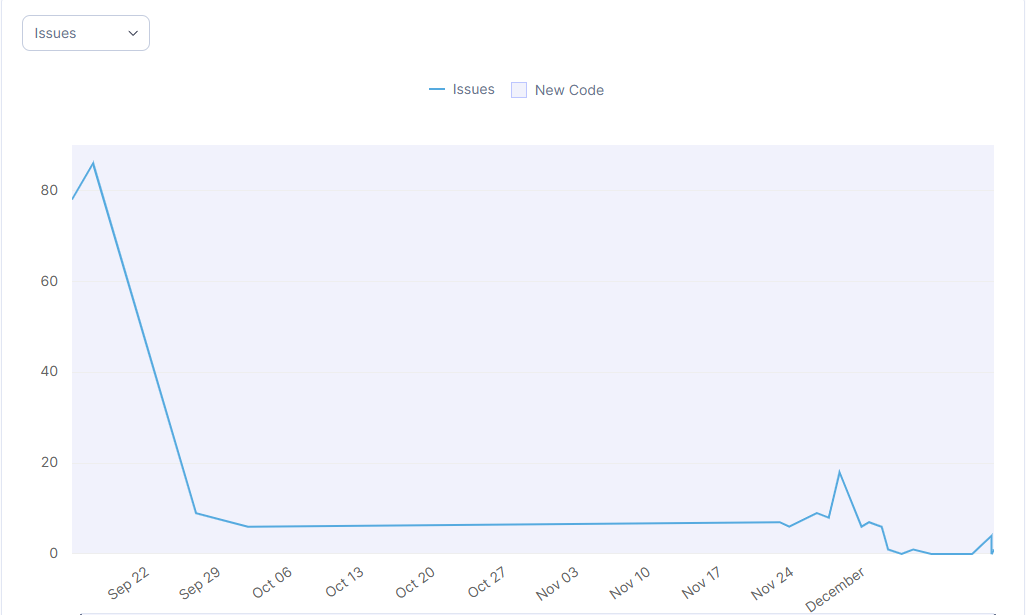
\includegraphics[width=0.7\linewidth]{Immagini/Verifica Software/Issues.png}
            \caption{Grafico dei code smells e dei bug}
        \end{figure} \\
        Il grafico sopra mostrato evidenzia i \textbf{bug} e i \textbf{code smells} nel codice, ossia delle abitudini o delle tecniche di scrittura dello stesso (definiti "pattern") che sfavoriscono la manutenibilità e/o la sicurezza. \\
        Sarebbe necessario mantenerne al minimo per cercare di ottenere un codice quanto più pulito possibile. \\
        Uno strumento che può correre in aiuto in tal senso è anche il plugin \textbf{SonarLint}, che si connette all'istanza in esecuzione di SonarQube sulla macchina per dare consigli on-the-fly per migliorare il codice, simili a quelli che fornirebbe un'analisi effettuata con SonarQube. \\
        \begin{figure}[htbp!]
            \centering
            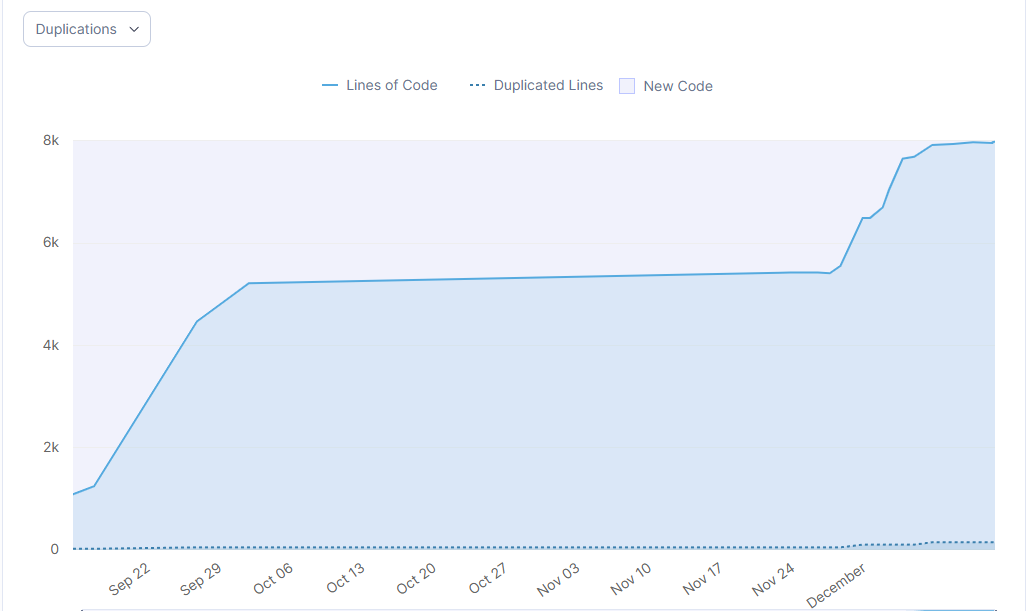
\includegraphics[width=0.7\linewidth]{Immagini/Verifica Software/Duplications.png}
            \caption{Grafico della duplicazione}
        \end{figure} \\
        Interessante è anche esaminare il grafico che mostra il livello di \textbf{duplicazione} nel codice. \\
        La linea blu continua mostra l'aumento della quantità delle righe di codice (asse delle ordinate, attualmente circa 8000 righe) nel tempo (asse delle ascisse). \\
        La linea tratteggiata, invece, mostra la quantità di righe che risultano duplicate all'interno del codice. \\
        Avere poche duplicazioni è essenziale considerando che sfavorisce la manutenibilità, in quanto in caso di modifica in un punto è necessaria una modifica anche negli altri punti, nonché la leggibilità, poiché allunga il corpo dei metodi nei quali viene inserito. \\
        Un livello così basso di duplicazione è stato ottenuto grazie a un attento \textbf{refactoring} del codice, ossia un'organizzazione altamente modulare dello stesso per favorire la futura evoluzione del software. \\
        \begin{figure}[htbp!]
            \centering
            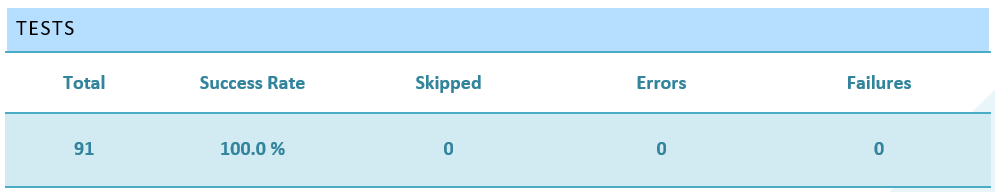
\includegraphics[width=0.7\linewidth]{Immagini/Verifica Software/Tests.png}
            \caption{Tabella dei test eseguiti}
        \end{figure} \\
        Osserviamo anche dal report di SonarQube le analisi dei test scritti per confermare il corretto funzionamento del software (sia Unit che Integration tests), appuntando come essi siano tutti risultati in un esito positivo. \\
        Prendiamo infine in esame il cruscotto riassuntivo del progetto nella dashboard di SonarQube, ove possiamo controllare la valutazione che lo strumento affibbia ad altre quattro qualità del software:
        \begin{itemize}
            \item \textbf{Sicurezza}, ossia problemi che possono comportare un accesso o un utilizzo non autorizzato dell backend dell'applicazione da parte di utenti malintenzionati;
            \item \textbf{Affidabilità}, ossia la capacità del codice di essere eseguito così come documentato gestendo i vari input e casi eccezionali senza causare crash o altri problemi;
            \item \textbf{Manutenibilità}, ossia la facilità di modifica del software nel caso di futuri sviluppi ed evoluzioni;
            \item \textbf{Hotspot di sicurezza}, ossia dei punti nei quali bisogna prestare particolare attenzione ai meccanismi di sicurezza per evitare utilizzo non consono o non autorizzato del software. \\
        \end{itemize}
        La valutazione per questi aspetti è, in una scala letterale americana, una "\textbf{A}", mostrando gli standard di qualità ai quali si attiene il codice, e tutti i punti caldi di sicurezza risultano revisionati e messi al sicuro. \\
        \begin{figure}[htbp!]
            \centering
            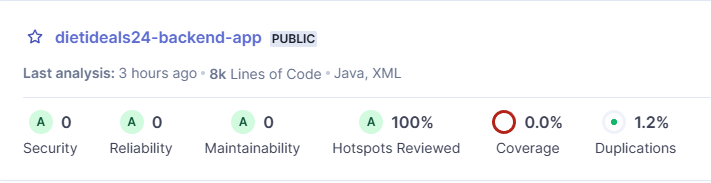
\includegraphics[width=0.7\linewidth]{Immagini/Verifica Software/Overall.png}
            \caption{Valutazione generale}
        \end{figure} \\

    \section{Verifica dinamica}
        La verifica dinamica è basata su tecniche di analisi dinamica del software, cioè per mezzo della sua esecuzione e osservandone il comportamento. Attraverso tecniche quali \textbf{testing} e \textbf{debugging} è possibile scovare i \textit{failure} ed individuarne i \textit{fault} che li hanno causati, così da correggerli. In particolare, il testing è stato effettuato attraverso la libreria \textbf{JUnit} sia su backend che su frontend (in quest'ultimo caso, un'implementazione apposita per Android).
        
        \subsection{I test: offertaService.checkFieldsValid (server)}
            Questo metodo verifica la validità dell'offerta inviata, verificando che i suoi attributi non violino le regole di business. \\
            
            \noindent La firma del metodo è la seguente:\\
            \texttt{void checkFieldsValid(OffertaDto offertaDto)} \\
            
            \noindent Dunque il metodo accetta un parametro di input, che tuttavia ha i seguenti attributi:
            \begin{itemize}
                \item \texttt{idOfferta}, che è un numero intero. Può essere qualsiasi valore;
                \item \texttt{dataInvio}, che è una data. Deve essere precedente alla data attuale;
                \item \texttt{oraInvio}, che è un orario. Se la data è precedente a quella attuale, può essere qualsiasi valore. Se la data è la stessa di quella attuale, deve essere precedente all'ora attuale
                \item \texttt{valore}, che è un numero decimale. Deve essere positivo \\
            \end{itemize}
            
            \noindent Si individuino le classi di equivalenza secondo un approccio basato per funzionalità.

            \begin{itemize}
                \item idOfferta:
                    \begin{itemize}
                        \item \textbf{C.E. 1:} idOfferta \textgreater{} 0;
                        \item \textbf{C.E. 2:} idOfferta = 0;
                        \item \textbf{C.E. 3:} idOfferta \textless{} 0;
                        \item \textbf{C.E. 4:} idOfferta = null.
                    \end{itemize}
                \item dataInvio:
                    \begin{itemize}
                        \item \textbf{C.E. 1:} dataInvio \textgreater{} data attuale;
                        \item \textbf{C.E. 2:} dataInvio = data attuale;
                        \item \textbf{C.E. 3:} dataInvio \textless{} data attuale;
                        \item \textbf{C.E. 4:} dataInvio = null.
                    \end{itemize}
                \item oraInvio:
                    \begin{itemize}
                        \item \textbf{C.E. 1:} oraInvio \textgreater{} ora attuale;
                        \item \textbf{C.E. 2:} oraInvio = ora attuale;
                        \item \textbf{C.E. 3:} oraInvio \textless{} ora attuale;
                        \item \textbf{C.E. 4:} oraInvio = null. \\
                    \end{itemize}
                \item valore:
                    \begin{itemize}
                        \item \textbf{C.E. 1:} valore \textgreater{} 0;
                        \item \textbf{C.E. 2:} valore = 0;
                        \item \textbf{C.E. 3:} valore \textless{} 0.
                        \item \textbf{C.E. 4:} valore = null.
                    \end{itemize}
            \end{itemize}

            \noindent Scegliamo di fare testing \textbf{Black-Box} con criterio di copertura per la combinazione di valori di tipo \textbf{R-WECT} (Robust - Weak Equivalence Class Testing).\\
            R-WECT prevede un totale di \(4+7 = 11\) tests, ovvero il più grande partizionamento (4 classi di equivalenza) più 6 casi non validi. Si scelga un valore da ciascuna classe di equivalenza.\\

            \noindent Per semplicità, esprimo i valori degli attributi del parametro in questo modo: \\
            \texttt{offertaDto\{idOfferta; dataInvio; oraInvio; valore\}}\\
            
            \noindent I test case sono:

            \begin{itemize}
                \item \texttt{checkFieldsValid(offertaDto\{5; LocalDate.now().minusDays(5); LocalTime.now().minusMinutes(5); BigDecimal.valueOf(1)\}} % 1 3 3 1
                \item \texttt{checkFieldsValid(offertaDto\{0; LocalDate.now(); LocalTime.now(); BigDecimal.valueOf(2)\}} % 2 2 2 1
                \item \texttt{checkFieldsValid(offertaDto\{-5; LocalDate.now().minusDays(5); LocalTime.now().plusMinutes(6); BigDecimal.valueOf(4)\}} % 3 3 1 1
                \item \texttt{checkFieldsValid(offertaDto\{null; LocalDate.now(); LocalTime.now().minusMinutes(6); BigDecimal.valueOf(4)\}} % 4 2 3 1
                \item \texttt{checkFieldsValid(offertaDto\{5; LocalDate.now(); LocalTime.now().plusMinutes(5);\\ BigDecimal.valueOf(1)\}} % 1 2 1 1
                \item \texttt{checkFieldsValid(offertaDto\{4; LocalDate.now().plusDays(3); LocalTime.now().minusMinutes(6); BigDecimal.valueOf(4)\}} % 1 1 2 1
                \item \texttt{checkFieldsValid(offertaDto\{4; null; LocalTime.now().minusMinutes(6); BigDecimal.valueOf(4)\}} % 1 4 2 1
                \item \texttt{checkFieldsValid(offertaDto\{4; LocalDate.now().minusDays(5); null; BigDecimal.valueOf(4)\}} % 1 3 4 1
                \item \texttt{checkFieldsValid(offertaDto\{5; LocalDate.now().minusDays(5); LocalTime.now().minusMinutes(5); BigDecimal.valueOf(0)\}} % 1 3 3 2
                \item \texttt{checkFieldsValid(offertaDto\{5; LocalDate.now().minusDays(5); LocalTime.now().minusMinutes(5); BigDecimal.valueOf(-5)\}} % 1 3 3 3
                \item \texttt{checkFieldsValid(offertaDto\{5; LocalDate.now().minusDays(5); LocalTime.now().minusMinutes(5); null\}} % 1 3 3 4
            \end{itemize}

            Ossia:

            \begin{lstlisting}[language=Java, caption=OffertaServiceTests.java]
    class OffertaServiceTests {

        private OffertaService offertaService;
    
        @BeforeEach
        void initUnderTest() {
            offertaService = new OffertaServiceImpl();
        }
    
        @Test
        void testCheckFieldsValid_idMaggioreDataMinoreOraMinoreValoreMaggiore() {
            // Arrange
            OffertaDto offertaDto = new OffertaDto();
            offertaDto.setIdOfferta(5L);
            offertaDto.setDataInvio(LocalDate.now().minusDays(5));
            offertaDto.setOraInvio(LocalTime.now().minusMinutes(5));
            offertaDto.setValore(BigDecimal.valueOf(1));
    
            // Act & Assert
            assertDoesNotThrow(() -> offertaService.checkFieldsValid(offertaDto));
        }
    
        @Test
        void testCheckFieldsValid_idZeroDataAttualeOraAttualeValoreMaggiore() {
            // Arrange
            OffertaDto offertaDto = new OffertaDto();
            offertaDto.setIdOfferta(0L);
            offertaDto.setDataInvio(LocalDate.now());
            offertaDto.setOraInvio(LocalTime.now());
            offertaDto.setValore(BigDecimal.valueOf(2));
    
            // Act & Assert
            assertDoesNotThrow(() -> offertaService.checkFieldsValid(offertaDto));
        }
    
        @Test
        void testCheckFieldsValid_idMinoreDataMinoreOraMaggioreValoreMaggiore() {
            // Arrange
            OffertaDto offertaDto = new OffertaDto();
            offertaDto.setIdOfferta(-5L);
            offertaDto.setDataInvio(LocalDate.now().minusDays(5));
            offertaDto.setOraInvio(LocalTime.now().plusMinutes(6));
            offertaDto.setValore(BigDecimal.valueOf(4));
    
            // Act & Assert
            assertDoesNotThrow(() -> offertaService.checkFieldsValid(offertaDto));
        }
    
        @Test
        void testCheckFieldsValid_idNullDataAttualeOraMinoreValoreMaggiore() {
            // Arrange
            OffertaDto offertaDto = new OffertaDto();
            offertaDto.setIdOfferta(null);
            offertaDto.setDataInvio(LocalDate.now());
            offertaDto.setOraInvio(LocalTime.now().minusMinutes(6));
            offertaDto.setValore(BigDecimal.valueOf(4));
    
            // Act & Assert
            assertDoesNotThrow(() -> offertaService.checkFieldsValid(offertaDto));
        }
    
        @Test
        void testCheckFieldsValid_idMaggioreDataAttualeOraMaggioreValoreMaggiore() {
            // Arrange
            OffertaDto offertaDto = new OffertaDto();
            offertaDto.setIdOfferta(5L);
            offertaDto.setDataInvio(LocalDate.now());
            offertaDto.setOraInvio(LocalTime.now().plusMinutes(5));
            offertaDto.setValore(BigDecimal.valueOf(1));
    
            // Act & Assert
            assertThrowsExactly(InvalidParameterException.class, () -> offertaService.checkFieldsValid(offertaDto));
        }
    
        @Test
        void testCheckFieldsValid_idMaggioreDataMaggioreOraMinoreValoreMaggiore() {
            // Arrange
            OffertaDto offertaDto = new OffertaDto();
            offertaDto.setIdOfferta(4L);
            offertaDto.setDataInvio(LocalDate.now().plusDays(3));
            offertaDto.setOraInvio(LocalTime.now().minusMinutes(6));
            offertaDto.setValore(BigDecimal.valueOf(4));
    
            // Act & Assert
            assertThrowsExactly(InvalidParameterException.class, () -> offertaService.checkFieldsValid(offertaDto));
        }
    
        @Test
        void testCheckFieldsValid_idMaggioreDataNullOraMinoreValoreMaggiore() {
            // Arrange
            OffertaDto offertaDto = new OffertaDto();
            offertaDto.setIdOfferta(4L);
            offertaDto.setDataInvio(null);
            offertaDto.setOraInvio(LocalTime.now().minusMinutes(6));
            offertaDto.setValore(BigDecimal.valueOf(4));
    
            // Act & Assert
            assertThrowsExactly(InvalidParameterException.class, () -> offertaService.checkFieldsValid(offertaDto));
        }
    
        @Test
        void testCheckFieldsValid_idMaggioreDataMinoreOraNullValoreMaggiore() {
            // Arrange
            OffertaDto offertaDto = new OffertaDto();
            offertaDto.setIdOfferta(4L);
            offertaDto.setDataInvio(LocalDate.now().minusDays(5));
            offertaDto.setOraInvio(null);
            offertaDto.setValore(BigDecimal.valueOf(1));
    
            // Act & Assert
            assertThrowsExactly(InvalidParameterException.class, () -> offertaService.checkFieldsValid(offertaDto));
        }
    
        @Test
        void testCheckFieldsValid_idMaggioreDataMinoreOraMinoreValoreZero() {
            // Arrange
            OffertaDto offertaDto = new OffertaDto();
            offertaDto.setIdOfferta(5L);
            offertaDto.setDataInvio(LocalDate.now().minusDays(5));
            offertaDto.setOraInvio(LocalTime.now().minusMinutes(5));
            offertaDto.setValore(BigDecimal.valueOf(0));
    
            // Act & Assert
            assertThrowsExactly(InvalidParameterException.class, () -> offertaService.checkFieldsValid(offertaDto));
        }
    
        @Test
        void testCheckFieldsValid_idMaggioreDataMinoreOraMinoreValoreMinore() {
            // Arrange
            OffertaDto offertaDto = new OffertaDto();
            offertaDto.setIdOfferta(5L);
            offertaDto.setDataInvio(LocalDate.now().minusDays(5));
            offertaDto.setOraInvio(LocalTime.now().minusMinutes(5));
            offertaDto.setValore(BigDecimal.valueOf(-5));
    
            // Act & Assert
            assertThrowsExactly(InvalidParameterException.class, () -> offertaService.checkFieldsValid(offertaDto));
        }
    
        @Test
        void testCheckFieldsValid_idMaggioreDataMinoreOraMinoreValoreNull() {
            // Arrange
            OffertaDto offertaDto = new OffertaDto();
            offertaDto.setIdOfferta(5L);
            offertaDto.setDataInvio(LocalDate.now().minusDays(5));
            offertaDto.setOraInvio(LocalTime.now().minusMinutes(5));
            offertaDto.setValore(null);
    
            // Act & Assert
            assertThrowsExactly(InvalidParameterException.class, () -> offertaService.checkFieldsValid(offertaDto));
        }
    }
            \end{lstlisting}
        

        \subsection{II test:  accountService.isEmailAndPasswordValid (server)}
            Questo metodo verifica la validità dell'email e password passati per parametro. \\
            
            \noindent La firma del metodo è la seguente:\\
            \texttt{boolean isEmailAndPasswordValid(String email, String password)} \\
            
            \noindent Dunque il metodo accetta due parametro di input:
            \begin{itemize}
                \item \texttt{email}, che è una stringa. Deve soddisfare la regex $\wedge[A-Za-z0-9+_.-]+@(.+)\textdollar$;
                \item \texttt{password}, che è una stringa. Deve essere non vuota.
            \end{itemize}
            
            \noindent Si individuino le classi di equivalenza secondo un approccio basato per funzionalità.

            \begin{itemize}
                \item email:
                    \begin{itemize}
                        \item \textbf{C.E. 1:} email = null;
                        \item \textbf{C.E. 2:} email = "";
                        \item \textbf{C.E. 3:} email rispetta l'espressione regolare;
                        \item \textbf{C.E. 4:} email non rispetta l'espressione regolare.
                    \end{itemize}
                \item password:
                    \begin{itemize}
                        \item \textbf{C.E. 1:} password = null;
                        \item \textbf{C.E. 2:} password = "";
                        \item \textbf{C.E. 3:} password è una qualsiasi stringa.
                    \end{itemize}
            \end{itemize}

            \noindent Scegliamo di fare testing \textbf{Black-Box} con criterio di copertura per la combinazione di valori di tipo \textbf{N-WECT} (Normal - Weak Equivalence Class Testing).\\
            N-WECT prevede un totale di \(4\) tests, ovvero il più grande partizionamento (4 classi di equivalenza). Si scelga un valore da ciascuna classe di equivalenza.\\
            
            \noindent I test case sono:

            \begin{itemize}
                \item \texttt{isEmailAndPasswordValid(null, null)} % 1 1
                \item \texttt{isEmailAndPasswordValid("", "")} % 2 2
                \item \texttt{isEmailAndPasswordValid("abc@def.it", "abc")} % 3 3
                \item \texttt{isEmailAndPasswordValid("abc", "")} % 4 2
            \end{itemize}

            \noindent Inoltre, in aggiunta al test Black-Box, ne facciamo anche uno di tipo \textbf{White-Box} con criterio di copertura per la combinazione di valori di tipo \textbf{branch coverage}. Prima di tutto, rappresentiamo il grafo del flusso di controllo della funzione:

            \begin{figure}[htbp!]
                \centering
                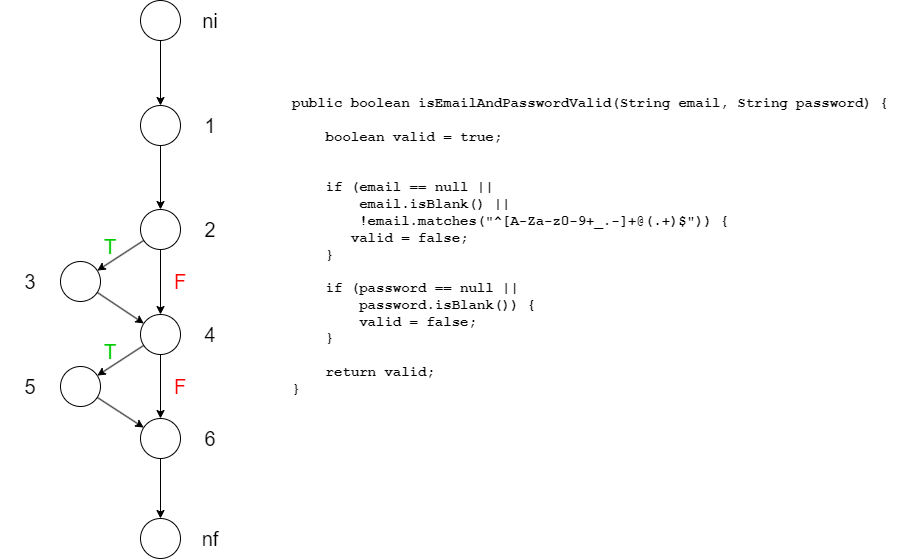
\includegraphics[width=0.5\linewidth]{Immagini/Verifica Software/Test WB isEmailAndPasswordValid.png}
                \caption{Grafo del flusso di controllo di isEmailAndPasswordValid}
            \end{figure}

            Si scelga un valore in modo da coprire ogni ramo.\\
            
            \noindent I test case sono:

            \begin{itemize}
                \item \texttt{isEmailAndPasswordValid("", null)} % 1 -> 2 -> 3 -> 4 -> 5 -> 6
                \item \texttt{isEmailAndPasswordValid("abc", "abc")} % 1 -> 2 -> 3 -> 4 -> 6
                \item \texttt{isEmailAndPasswordValid("abc@def.it", null)} % 1 -> 2 -> 4 -> 5 -> 6
                \item \texttt{isEmailAndPasswordValid("ABc@CDe.A", "123")} % 1 -> 2 -> 4 -> 6
            \end{itemize}

            Ossia:

            \begin{lstlisting}[language=Java, caption=AccountServiceTests.java]
    class AccountServiceTests {
    
        @MockBean
        private TokensAccountMapper tokensAccountMapper;
    
        @MockBean
        private RelationsConverter relationsConverter;
    
        @MockBean
        private AccountRepository accountRepository;
    
    
        private AccountServiceImpl accountService;
    
        @BeforeEach
        void initUnderTest() {
            this.accountService = new AccountServiceImpl(tokensAccountMapper, relationsConverter, accountRepository);
        }
    
        // Test Black-Box
        @Test
        void testIsEmailAndPasswordValid_EmailNullPasswordNull() {
            // Arrange
            String email = null;
            String password = null;
    
            boolean result = accountService.isEmailAndPasswordValid(email, password);
    
            // Act
            boolean oracolo = false;
    
            // Assert
            assertEquals(oracolo, result);
        }
    
        @Test
        void testIsEmailAndPasswordValid_EmailBlankPasswordBlank() {
            // Arrange
            String email = "";
            String password = "";
    
            boolean result = accountService.isEmailAndPasswordValid(email, password);
    
            // Act
            boolean oracolo = false;
    
            // Assert
            assertEquals(oracolo, result);
        }
    
        @Test
        void testIsEmailAndPasswordValid_EmailValidPasswordValid_1() {
            // Arrange
            String email = "abc@def.it";
            String password = "abc";
    
            boolean result = accountService.isEmailAndPasswordValid(email, password);
    
            // Act
            boolean oracolo = true;
    
            // Assert
            assertEquals(oracolo, result);
        }
    
        @Test
        void testIsEmailAndPasswordValid_EmailNotValidPasswordBlank() {
            // Arrange
            String email = "abc";
            String password = "";
    
            boolean result = accountService.isEmailAndPasswordValid(email, password);
    
            // Act
            boolean oracolo = false;
    
            // Assert
            assertEquals(oracolo, result);
        }
    
        // Test White-Box
        @Test
        void testIsEmailAndPasswordValid_EmailBlankPasswordNull() {
            // Arrange
            String email = "";
            String password = null;
    
            boolean result = accountService.isEmailAndPasswordValid(email, password);
    
            // Act
            boolean oracolo = false;
    
            // Assert
            assertEquals(oracolo, result);
        }
    
        @Test
        void testIsEmailAndPasswordValid_EmailNotValidPasswordValid() {
            // Arrange
            String email = "abc";
            String password = "abc";
    
            boolean result = accountService.isEmailAndPasswordValid(email, password);
    
            // Act
            boolean oracolo = false;
    
            // Assert
            assertEquals(oracolo, result);
        }
    
        @Test
        void testIsEmailAndPasswordValid_EmailValidPasswordNull() {
            // Arrange
            String email = "abc@def.it";
            String password = null;
    
            boolean result = accountService.isEmailAndPasswordValid(email, password);
    
            // Act
            boolean oracolo = false;
    
            // Assert
            assertEquals(oracolo, result);
        }
    
        @Test
        void testIsEmailAndPasswordValid_EmailValidPasswordValid_2() {
            // Arrange
            String email = "ABc@CDe.A";
            String password = "123";
    
            boolean result = accountService.isEmailAndPasswordValid(email, password);
    
            // Act
            boolean oracolo = true;
    
            // Assert
            assertEquals(oracolo, result);
        }
    }
            \end{lstlisting}


        \subsection{III test: ModelProfilo validate (client)}
            Questo metodo verifica, quando si modifica il profilo, che i campi obbligatori non siano non validi. \\

            \noindent La firma del metodo è la seguente:\\
            \texttt{fun validate(nome: String, cognome: String, dataNascita: LocalDate)} \\

            \noindent Dunque il metodo accetta tre parametri di input:
            \begin{itemize}
                \item\texttt{nome}, una stringa che rappresenta un nome;
                \item\texttt{cognome}, una stringa che rappresenta un cognome;
                \item\texttt{dataNascita}, che rappresenta una data. \\
            \end{itemize}

            \noindent Si individuino le classi di equivalenza secondo un approccio basato per funzionalità.

            \begin{itemize}
                \item nome:
                    \begin{itemize}
                        \item\textbf{C.E. 1:} nome vuoto;
                        \item\textbf{C.E. 2:} nome compilato;
                    \end{itemize}
                \item cognome:
                    \begin{itemize}
                        \item\textbf{C.E. 1:} cognome vuoto;
                        \item\textbf{C.E. 2:} cognome compilato;
                    \end{itemize}
                \item dataNascita:
                    \begin{itemize}
                        \item\textbf{C.E. 1:} dataNascita = LocalDate.MIN;
                        \item\textbf{C.E. 2:} dataNascita != LocalDate.MIN; 
                    \end{itemize}
            \end{itemize}

            \noindent Scegliamo di fare testing \textbf{Black-Box} con criterio di copertura per la combinazione di valori di tipo \textbf{N-SECT} (Normal - Strong Equivalence Class Testing).\\
            N-SECT prevede un totale di \(2*2*2 = 8\) tests, ovvero il prodotto cartesiano tra tutte le classi di equivalenza. Si scelga un valore da ciascuna classe di equivalenza. \\
            
            \noindent I test case sono:

            \begin{itemize}
                \item\texttt{validate("", "", LocalDate.MIN)} % Tutti errati
                \item\texttt{validate("Mario", "Rossi", LocalDate.of(1980,6,5)} % Tutti giusti
                \item\texttt{validate("", "Rossi", LocalDate.of(1980,6,5))} % Nome errato
                \item\texttt{validate("Mario", "", LocalDate.of(1980,6,5))} % cognome errato
                \item\texttt{validate("Mario", "Rossi", LocalDate.MIN)} % Data nascita errata
                \item\texttt{validate("", "", LocalDate.of(1980,6,5))} % Nome e cognome errati
                \item\texttt{validate("", "Rossi", LocalDate.MIN)} % Nome e data nascita errati
                \item\texttt{validate("Mario", "", LocalDate.MIN)} % Cognome e data nascita errati
            \end{itemize}

            Ossia:

            \begin{lstlisting}[language=Java, caption=ModelProfiloTests.java]
    @RunWith(AndroidJUnit4.class)
    public class ModelProfiloTests {
    
        private ModelProfilo viewModel;
    
        @Before
        public void setup() {
            viewModel = new ModelProfilo();
        }
    
        @Test
        public void test_TuttiMancanti() {
            assertThrows(EccezioneCampiNonCompilati.class, () -> viewModel.validate("", "", LocalDate.MIN));
        }
    
        @Test
        public void test_TuttiCompilati() {
            try {
                viewModel.validate("Mario", "Rossi", LocalDate.of(1980, 6, 5));
            } catch (EccezioneCampiNonCompilati e) {
                fail();
            }
        }
    
        @Test
        public void test_NomeMancante() {
            assertThrows(EccezioneCampiNonCompilati.class, () -> viewModel.validate("", "Rossi", LocalDate.of(1980, 6, 5)));
        }
    
        @Test
        public void test_CognomeMancante() {
            assertThrows(EccezioneCampiNonCompilati.class, () -> viewModel.validate("Mario", "", LocalDate.of(1980, 6, 5)));
        }
    
        @Test
        public void test_DataNascitaMancante() {
            assertThrows(EccezioneCampiNonCompilati.class, () -> viewModel.validate("Mario", "Rossi", LocalDate.MIN));
        }
    
        @Test
        public void test_NomeECognomeMancanti() {
            assertThrows(EccezioneCampiNonCompilati.class, () -> viewModel.validate("", "", LocalDate.of(1980, 6, 5)));
        }
    
        @Test
        public void test_NomeEDataNascitaMancanti() {
            assertThrows(EccezioneCampiNonCompilati.class, () -> viewModel.validate("", "Rossi", LocalDate.MIN));
        }
    
        @Test
        public void test_CognomeEDataNascitaMancanti() {
            assertThrows(EccezioneCampiNonCompilati.class, () -> viewModel.validate("Mario", "", LocalDate.MIN));
        }
    }
            \end{lstlisting}
            
        \subsection{IV test: JWTTests getUserEmail (client)}
            Questo metodo estrae, quando è stato recuperato l'access token dall'authentication server di Cognito, l'email dell'utente che ha effettuato l'accesso o la registrazione. \\
            Decodifica prima il JWT dalla base 64 e poi estrapola con l'aiuto di una espressione regolare e un gruppo di cattura il valore dell'email. \\

            \noindent La firma del metodo è la seguente:\\
            \texttt{fun getUserEmail(jwt: String): String} \\

            \noindent Dunque il metodo restituisce l'email sotto forma di stringa e accetta un parametro di input:
            \begin{itemize}
                \item\texttt{jwt}, una stringa che contiene l'intero JWT recuperato da Cognito. \\
            \end{itemize}

            \noindent Si individuino le classi di equivalenza secondo un approccio basato per funzionalità.

            \begin{itemize}
                \item jwt:
                    \begin{itemize}
                        \item\textbf{C.E. 1:} il JWT contiene l'email dell'utente;
                        \item\textbf{C.E. 2:} il JWT non contiene l'email dell'utente;
                        \item\textbf{C.E. 3:} il JWT è vuoto; \\
                    \end{itemize}
            \end{itemize}

            \noindent Consideriamo adesso tutti i valori che la stringa può assumere.\\
            
            \noindent I test case sono:

            \begin{itemize}
                \item\texttt{getUserEmail("eyJhbGciOiJIUzI1NiIsInR5cCI6IkpXVCJ9.eyJlbWFpbCI6InRlc3RAdGVzdC5jb20ifQ.sig")} % JWT con email
                \item\texttt{getUserEmail("eyJhbGciOiJIUzI1NiIsInR5cCI6IkpXVCJ9.eyJzdWIiOiIxMjM0NTY3ODkwIn0.sig")} % JWT senza email
                \item\texttt{getUserEmail("")} % JWT vuoto
            \end{itemize}

            Ossia:

            \begin{lstlisting}[language=Java, caption=JWTTests.java]
    @RunWith(AndroidJUnit4.class)
    public class JWTTests {
    
        @Test
        public void test_emailPresente() {
            String jwt = "eyJhbGciOiJIUzI1NiIsInR5cCI6IkpXVCJ9.eyJlbWFpbCI6InRlc3RAdGVzdC5jb20ifQ.sig";
            String email = JWT.Companion.getUserEmail(jwt);
            assertEquals("test@test.com", email);
        }
    
        @Test
        public void test_emailAssente() {
            String jwt = "eyJhbGciOiJIUzI1NiIsInR5cCI6IkpXVCJ9.eyJzdWIiOiIxMjM0NTY3ODkwIn0.sig";
            String email = JWT.Companion.getUserEmail(jwt);
            assertEquals("", email);
        }
    
        @Test
        public void test_jwtVuoto() {
            String jwt = "";
            String email = JWT.Companion.getUserEmail(jwt);
            assertEquals("", email);
        }
    }
            \end{lstlisting}